\documentclass[12pt]{article}
\usepackage[a4paper, margin=.30in]{geometry}
\usepackage{graphicx ,
            wrapfig,
            xcolor, 
            enumerate,
            amsmath,fontenc, mhchem,makecell
            }

\newcommand\headerMe[2]{\noindent{}#1\hfill#2}
\renewcommand{\thesection}{\Roman{section}}

\author{Zakaria HAOUZAN}
\date{\today}

\begin{document}
% headers --------------
\headerMe{Matière : Physique-Chimie}{Professeur : Zakaria HAOUZAN}\\
\headerMe{Unité : Transformations non totales d'un\\système chimique  }{Établissement : Lycée SKHOR qualifiant}\\
\headerMe{Niveau : 2BAC-SM-PC}{Heure : 3H}\\

% ------Content ________
\begin{center}

    \Large{Leçon $N^{\circ} 3.1 $: \color{red} Transformations chimiques qui ont lieu dans les deux sens. }
\end{center}

%\begin{figure}[h!]
	%\begin{center}
	%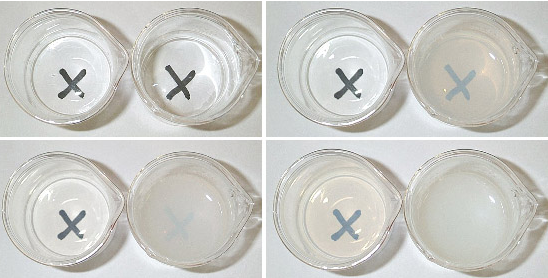
\includegraphics[width=0.5\textwidth]{./img/TRLconcentration.png}
%\end{center}
%\vspace{-1cm}
%\end{figure}



%\begin{wrapfigure}[10]{r}{0.5\textwidth}
%    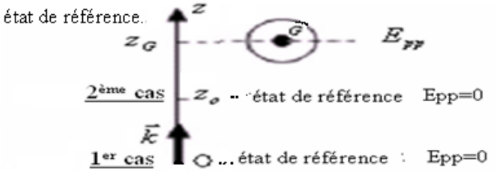
\includegraphics[width=0.5\textwidth]{./img/img00.png}
%\end{wrapfigure}


%\begin{center}
   %\begin{tabular}{|c|c|c|}
      %\hline
      %Indicateur coloré & Couleur de l’espèce acide & Couleur de l’espèce base\\\hline
      %BBT               & Jaune                     & Bleue\\\hline
      %Hélianthine       &Rose                       & Jaune\\\hline
      %Phénolphtaléine   & inclore                   & rose \\\hline
   %\end{tabular}
%\end{center}

\section{Réactions acide-Base}

\subsection{Définition de Bronsted}
On appelle acide de Bronsted toute espèce chimique capable de céder un proton $H^+$ pendant une transformation chimique.

On appelle base de Bronsted toute espèce chimique capable de capter un proton $H^+$ pendant une transformation chimique.


\subsection{Notion de couple acide-base : }
Un couple acide/Base (noté A/B) est constitué d'un acide A et sa base conjugée B qui généralement liés par la demi-équation: \ce{A <--> $H^+$ + B}

Exemples de quelques couples acide-base : $CH_3COOH/CH_3COO^-$ ; $NH_4^+/NH_3$ ; $H_3O^+/H_2O$

\subsection{Réactions acide-base :}
Au cours d’une réaction acido-basique il y’a échange d'un proton $H^+$  entre deux couples acide-base :$A_1/B_1$ et $A_2/B_2$
L'équation de la réaction entre l'acide A1 du 1er couple et la base B2 du 2ème couple s'écrit :$$\ce{A_1 <=>B_1 + H^+}$$
$$\ce{B_2 + H^+ <=>A_2}$$

Exemple :Ecrire l'équation de la réaction acide-base entre l'acide du couple $CH_3COOH/CH_3COO^-$ et la base du couple $NH4^+/NH_3$.

\section{Introduction de la notion pH : }

\subsection{Définition:}
Les propriétés acido-basique d'une solution aqueuse dépendent de la concentration des ions oxonium $H_3O^+$ liée au pH de la solution par la relation suivante : $$pH = -log[H_3O^+]  <=> [H_3O^+] = 10^{-pH}$$
Le pH est une grandeur sans unité.

\subsection{Mesure du pH : }

\begin{wrapfigure}{r}{0.33\textwidth}
	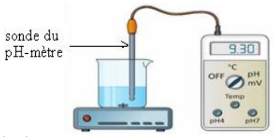
\includegraphics[width=0.33\textwidth]{./img/phMesure.png}
\end{wrapfigure}


Pour mesurer le pH d'une solution on utilise le pH-mètre qui se compose d'une sonde de mesure reliée à un voltmètre
électronique gradué en unité de pH. On doit étalonner le pH-mètre avant toute mesure.

\section{Avancement d'une réaction chimique:  }
\subsection{Avancement final et l'avancement maximal : }
L'avancement d'une réaction est la quantité de matière x des réactifs qui disparait ou des produits qui se forme selon
les coefficients stœchiométriques.

L'avancement maximal $x_{max}$ est l'avancement qui correspond à la disparition du réactif limitant.

L'avancement final $x_f$ est la valeur de l'avancement qui correspond à l'état final d'une réaction limitée.

\subsection{ Le taux d'avancement final d'une réction chimique:}
Le taux d'avancement finale d'une réction chimique est le quotient de l'avancement final par l'avancement maximal. 

$0 \leq \tau \leq 1$ Pour cette raison on l'exprime souvent en pourcentag \%.
$$\tau = \frac{x_f}{x_{max}}$$ 

Le taux d'avancement est une grandeur sans unité.

\begin{itemize}
	\item si $\tau$ = 1 ; $x_f = x_{max}$ donc la réaction est totale.
	\item si $\tau < 1$ ; $x_f < x_{max}$ la réaction est limitée.
\end{itemize}
\subsection{Détermination éxpérimentale du taux d'avancement final :}
On introduit dans un bécher un volume $V=500cm^3$ d'eau distillée et on lui ajoute un volume $V=1cm^3$ d'une solution d'acide éthanoïque pure.

On mesure de le pH du mélange à l'aide d'un pH mètre et on obtient : pH=3,1.

La réaction de l'acide éthanoïque avec l'eau s'écrit:
$\ce{CH_3COOH + H_2O -> CH_3COO^- + H_3O^+} $

La densité de l'acide éthanoïque : d=1,05;

La masse volumique de l'eau : $\rho_{eau} = 1g/cm^3$.

La masse molaire de la molécule d'acide éthanoïque:$M(CH_3COOH) = 60g/mol$

1) Déterminer la quantité de matière initiale de l'acide éthanoïque.

2) Dresser le tableau d'avancement de la réaction puis déterminer la valeur de l'avancement maximal.

4) Déterminer la valeur de l'avancement final. Quelle est votre conclusion.

5) Calculer le taux d'avancement final de la réaction.

\section{Equilibre chimique d'un système chimique : }

Les ions éthanoate $CH_3COO^-$ réagissent avec les ions oxoniums $H_3O^+$ et cette réaction est aussi une réaction limitée. 
$$\ce{ CH_3COO^- + H_3O^+ -> CH_3COOH + H_2O } $$
C'est la réaction inverse de celle de l'acide éthanoïque avec l'eau. Ces deux réactions se produisent en même temps et conduisent à
un équilibre chimique qu'on symbolise par deux flèches:
$$\ce{CH_3COOH + H_2O <=>[1][2] CH_3COO^- + H_3O^+} $$
Lorsque l'équilibre chimique est atteint, les quantités de matière des réactifs et des produits ne varient pas et le
système n'évolue plus. C'est ce qu'on appelle un état d'équilibre dynamique.
On constate ceci à partir du tableau d'avancement.

\begin{tabular}{|c|c|c|c|c|c|}
    \hline
    \multicolumn{2}{|c|}{Equation de la réaction}& \multicolumn{4}{c|}{
\ce{CH_3COOH + H_2O <=>[1][2] CH_3COO^- + H_3O^+}}\\\hline
    états  & avancement& \multicolumn{4}{|c|}{quantité de Matière en mol}\\\hline
	Etat initial          &    0        &  $1,75.10^{-2}$ &  - &  0              &  0 \\\hline
                 \makecell{Etat de \\transformation}&    $x$      & $1,75.10^{-2}-x$ & - & $x$  & $x$ \\\hline
				 Etat final            & $x_f=4.10^{-4}$ & $n_i - n_f = 1,71.10^{-2}$ & -  & $4.10^{-4}$&$4.10^{-4}$ \\\hline
   % \cline{2-4}\
\end{tabular}

Lorsque l'équilibre  est atteint la réaction apparait comme s'elle n'évolue plus.

Pour toute transformation limitée, l'écriture de l'équation chimique s'écrit avec deux flèches: \ce{ <=> }

Car la transformation est décrite microscopiquement par deux réactions inverses l'une de l'autre.

\subsection{Interpretation microscopique de l'état d'équilibre d'un système : }
On considère le système chimique : $\ce{A + B <=>[1][2] C + D}$.

A l'état initial le système contient les espèces chimiques A et B, la réaction se produit dans le sens (1) avec la vitesse v1.

Au cours du temps l'avancement augmente , par conséquence :
\begin{itemize}

	\item Les quantités des espèces A et B ainsi que les chocs entre elles diminuent donc diminution de v1.
	\item  Les espèces C et D apparaissent et la réaction se produit dans le sens (2) avec la vitesse v2 leur quantité ainsi que les chocs entre elles augmentent donc augmentation de v2.

	\item Lorsque les deux vitesses v1 et v2 s'égalisent: le système n'évolue plus.C'est l'état d'équilibre.
Au niveau macroscopique le système ne semble pas évoluer
\end{itemize}
\section{Exercice d'application:}
On considère une solution S d'acide benzoïque .L'équation de sa réaction avec l'eau s'écrit: 

$\ce{C_6H_5COOH + H_2O <=> C_6H_5COO^- + H_3O^+}$

La mesure de sa conductivité a donné la valeur suivante: $\sigma = 36,1 mS/m$.

1) Dresser le remplissage du tableau d'avancement suivant:

2) Donner l'expression de la conductivité $\sigma $ du mélange réactionnel en fonction de $\lambda_{H_3O^+}$ ; $\lambda_{C_6H_5COO^-}$  du volume V de la solution et l'avancement final $x_f$.

3) Déterminer la valeur de l'avancement final de la dissociation de l'acide benzoïque dans l'eau.

On donne: $\lambda_{H_3O^+} = 35 mS.m^2/mol$ ; $\lambda_{C_6H_5COO^-} = 3,23 mS.m^2/mol$

4) En déduire les concentrations molaires finales de $H_3O^+$ et $C_6H_5COO^-$.

5) Calculer le pH de la solution obtenue .

6) Déterminer le taux d'avancement final sachant que la concentration de la solution est : 
$C=1,18.10^{-2}mol/L$

\end{document}
